%%%%%%%%%%%%%%%%%%%%%%%%%%%%%%%%%%%%%%%%%%%%%%%%%%%%%%%%%%%%%%%%%%
%%%%%%%% ICML 2011 EXAMPLE LATEX SUBMISSION FILE %%%%%%%%%%%%%%%%%
%%%%%%%%%%%%%%%%%%%%%%%%%%%%%%%%%%%%%%%%%%%%%%%%%%%%%%%%%%%%%%%%%%

\def\S{K}
\def\reals{\mathbb{R}}
\def\tr{\mathrm{tr}}
\def\cS{\mathcal{S}}
\def\cL{\mathcal{L}}
\def\U{\mathcal{U}}
\def\hp{\hat{p}}
\newtheorem{theorem}{Theorem}

% Use the following line _only_ if you're still using LaTeX 2.09.
%\documentstyle[icml2011,epsf,natbib]{article}
% If you rely on Latex2e packages, like most moden people use this:
\documentclass{article}

% For figures
\usepackage{graphicx} % more modern
%\usepackage{epsfig} % less modern
\usepackage{subfigure}
\usepackage{sidecap}

% For citations
\usepackage{natbib}

% For algorithms
\usepackage{algorithm}
\usepackage{amsfonts}
\usepackage{algorithmic}

% As of 2010, we use the hyperref package to produce hyperlinks in the
% resulting PDF.  If this breaks your system, please commend out the
% following usepackage line and replace \usepackage{icml2011} with
% \usepackage[nohyperref]{icml2011} above.
\usepackage{hyperref}

% Packages hyperref and algorithmic misbehave sometimes.  We can fix
% this with the following command.
\newcommand{\theHalgorithm}{\arabic{algorithm}}

% Employ the following version of the ``usepackage'' statement for
% submitting the draft version of the paper for review.  This will set
% the note in the first column to ``Under review.  Do not distribute.''
\usepackage{icml2011}
% Employ this version of the ``usepackage'' statement after the paper has
% been accepted, when creating the final version.  This will set the
% note in the first column to ``Appearing in''
% \usepackage[accepted]{icml2011}


% The \icmltitle you define below is probably too long as a header.
% Therefore, a short form for the running title is supplied here:
\icmltitlerunning{Actively Learning the Crowd Kernel}

\begin{document}

\twocolumn[
\icmltitle{Adaptively Learning the Crowd Kernel}


% It is OKAY to include author information, even for blind
% submissions: the style file will automatically remove it for you
% unless you've provided the [accepted] option to the icml2011
% package.
\icmlauthor{Your Name}{email@yourdomain.edu}
\icmladdress{Your Fantastic Institute,
            314159 Pi St., Palo Alto, CA 94306 USA}
\icmlauthor{Your CoAuthor's Name}{email@coauthordomain.edu}
\icmladdress{Their Fantastic Institute,
            27182 Exp St., Toronto, ON M6H 2T1 CANADA}

% You may provide any keywords that you
% find helpful for describing your paper; these are used to populate
% the "keywords" metadata in the PDF but will not be shown in the document
\icmlkeywords{active learning, crowdsourcing, kernels}

\vskip 0.3in
]

\begin{abstract}
  We introduce an algorithm that, given $n$ objects, learns a similarity matrix over all $n^2$
  pairs, from crowdsourced data alone.  The algorithm samples responses to
  {\em adaptively chosen} triplet-based relative-similarity queries.  Each query has the form
  ``is object $a$ more similar to $b$ or to $c$?'' and is chosen to be
  maximally informative given the preceding responses.  The output is
  an embedding of the objects into Euclidean space (like MDS); we refer to this
  as the ``crowd kernel.''  

  The runtime (empirically observed to be linear) and cost (about
  \$0.15 per object) of the algorithm are small enough to permit its
  application to databases of thousands of objects.  The distance
  matrix provided by the algorithm allows for the development of an
  intuitive and powerful sequential, interactive search algorithm
  which we demonstrate for a variety of visual stimuli.  We present
  quantitative results that demonstrate the benefit in cost and time
  of our approach compared to a nonadaptive approach.  We also show
  the ability of our approach to capture different aspects of
  perceptual similarity by demonstrating a variety of binary attribute
  classifiers (``is striped,'' ``vowel vs.\ consonant'') trained
  using the learned kernel.  

\end{abstract}

\section{Introduction}
The problem of capturing and extrapolating a human notion of
perceptual similarity has received increasing attention in recent
years including areas such as vision \cite{Agarwal07}, audition \cite{McFee09}, information
retrieval \cite{Schultz03} and a variety of others represented in the
UCI Datasets \cite{Xing02,Huang10}.  Concretely, the goal of these
approaches is to estimate a similarity matrix $K$ over all pairs of
$n$ objects given a (potentially exhaustive) subset of human
perceptual measurements on tuples of objects.  In some cases the set
of human measurements represents `side information' to computed
descriptors (MFCC, SIFT, etc.), while in other cases -- the present
work included -- one proceeds exclusively with human reported data.  
When $K$ is a positive semidefinite matrix induced purely from distributed human
measurements, we refer to it as the {\em crowd kernel} for the set of
objects.

Given such a Kernel, one can exploit it for a variety of purposes
including exploratory data analysis or embedding visualization (as in
Multidimensional Scaling) and relevance-feedback based interactive
search.  As discussed in the above works and \cite{Kendall90}, using a
{\em triplet based} representation of relative similarity, in which a
subject is asked ``is object $a$ more similar to $b$ or to $c$,'' has
a number of desirable properties over the classical approach employed
in Multi-Dimensional Scaling (MDS), i.e., asking for a numerical estimate of ``how similar is
object $a$ to $b$.''  These advantages include reducing fatigue on
human subjects and alleviating the need to reconcile individuals'
scales of similarity.  The obvious drawback with the triplet
based method, however, is the potential $O(n^3)$ complexity.  It is
therefore expedient to seek methods of obtaining high quality
approximations of $K$ from as small a subset of human measurements as
possible.   Accordingly, the primary contribution of this paper is an 
efficient method for estimating $K$ via an information theoretic 
adaptive sampling approach.


\begin{figure}
\center{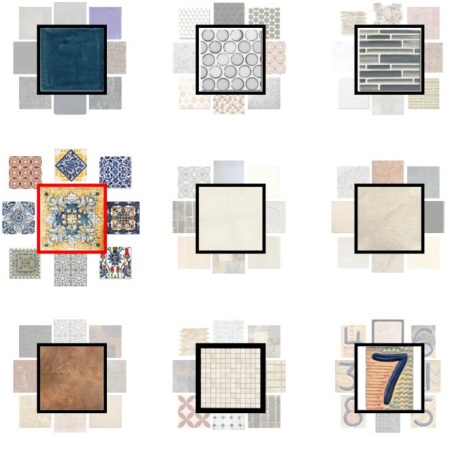
\includegraphics[width=3in]{tiles-tree-top.pdf}} \caption{\label{fig:tilestree} A sample top-level of a similarity search system that enables a user to search for objects by similarity.  In this case, since the user clicked on the middle-left tile, she will ``zoom-in'' and be presented with similar tiles.}
\end{figure}

At the heart of our approach is a new scale-invariant Kernel approximation model.  The choice of Kernel approximation model is shown to be crucial in terms of the adaptive triples that are produced, and the new model produces effective triples to label.  Although this model is nonconvex, we prove that it can be optimized under certain assumptions.  

We construct an end-to-end system for interactive visual search and
browsing using our Kernel acquisition algorithm. The input to this
system is a set of images of objects, such as products available in an
online store. The system automatically crowdsources the kernel
acquisition and then uses this kernel to produce a visual interface
for searching or browsing the set of products. Figure
\ref{fig:tilestree} shows this interface for a dataset of 433 floor
tiles available at amazon.com.

\subsection{Human kernels versus machine kernels}
The bulk of work in Machine Learning focuses on ``Machine Kernels''
that are computed by computer from the raw data (e.g., pixels)
themselves.  Additional work employs human experiments to try to learn
kernels based upon machine features, i.e., to approximate the human
similarity assessments based upon features that can be derived by
machine.  In contrast, when a kernel is learned from human subjects
alone (whether it be data from an individual or a crowd) one requires
no machine features whatsoever. To the computer, the objects
are recognized by ID's only -- the images themselves are hidden from
our system and are only presented to humans.

The primary advantage of machine kernels is that they can generalize immediately to new data, whereas each additional object needs to be added to our system, for a cost of approximately \$0.15.  On the other hand, working with a human kernel has two primary advantages.  First, it does not require any domain expertise.  While for any particular domain, such as music or images of faces, cars, or sofas, decades of research may have provided high-quality features, one does not have to find, implement, and tune these sophisticated feature detectors.  

Second, human kernels may contain features that are simply not available with state-of-the-art feature detectors, because of knowledge and experience that humans possess.  For example, from images of celebrities, human similarity may be partly based on whether the two celebrities are both from the same profession, such as politicians, actors, and so forth.  Until the longstanding goal of bridging the semantic gap is achieved, humans will be far better than machines at interpreting a number of features, such as ``does a couch look comfortable,'' ``can a shoe be worn to an informal occasion,'' or ``is a joke funny.''

We give a simple demonstration of external knowledge through
experiments on 26 images of the lower-case Roman alphabet.  Here, the
learned Kernel is shown to capture features such as ``is a letter
a vowel versus consonant,'' which uses
external knowledge beyond the pixels.  Note that this experiment is
interesting in itself because it is not at first clear if people can
meaningfully answer the question: ``is the letter {\em e} more similar
to {\em i} or {\em p}.'' Our experiments show statistically significant consistency with 58\%
($\pm$2\%, with 95\% confidence) agreement between users on a random
triple of letters.  (For random image triples from an online tie
store, 68\% agreement is observed, and 65\% is observed for floor tile images).


\section{Benefits of adaptation}
We first give high-level intuition for why adaptively choosing triples may 
yield better kernel approximations than randomly choosing triples.  
First consider a dataset of $n$ objects that naturally partitions into 
$k \ll n$ disjoint equal-sized
clusters, such that between clusters objects are completely dissimilar
but within clusters they have varied similarities.  For example, our
images from an online tie store cluster into ties, tie clips, and
scarves.  Say that, within any specific cluster, one can locate the object using $q$
queries by comparing it to other objects in the same cluster.  On the
other hand, suppose comparisons with objects in two different classes
simply yield 50/50 random results if the three objects are in
different classes but that the crowd will select an object of the same
class if one exists in the comparison pair.  The number of adaptive
queries to learn in such a setting is $\Theta(nk+nq)$: $\Theta(k)$
comparisons are required to determine which class each object is in
(with high probability) and then an additional $q$ queries are
required.  With random queries, one would require $\Theta(n k^2 q)$
queries, because only a $1/k^2$ fraction of the random queries will
count towards the $q$ necessary queries within objects of the same
class.


Next, consider data representing an underlying rooted tree with $k \ll n$ leaves, inspired by, say, phylogenic trees involving animal species.\footnote{This example is based upon a tree metric rather than a Euclidean one.  However, note that any tree with $k$ leaves can be embedded in $k$-dimensional Euclidean space so that the squared distance between any pair of embedded points is equal to the number of edges in their shortest path on the tree.  Moreover, the rich study of Embeddings (see, e.g., \citealp{IM04}) has shown that many types of metrics can be embedded (to varying degrees of approximation) within Euclidean space.}  Say the similarity between objects is decreasing in their distance in the tree graph and, furthermore, that objects are drawn uniformly at random from the classes represented by the leaves of the tree.  Ignoring the details of how one would identify that two objects are in the same leaf or subtree, it is clear that a nonadaptive method would have to ask $\Omega(n k)$ questions to determine the leaves to which $n$ objects belong (or at least to determine which objects are in the same tree).  On the other hand, in an ideal setting, an adaptive approach might determine such matters using $O(n \log k)$ queries in a balanced binary tree, assuming a constant number of comparisons can determine to which subtree of a node an object belongs, hence an exponential savings.

\section{Related work}

As discussed above, much of the work in machine learning on learning kernels employs `side information' in the form of features about objects.  \citet{Schultz03} highlight the fact that triple-based information may also be gathered by web search click data.
\citet{Agarwal07} is probably the most similar work, in which they learn a kernel matrix from triples of similarity comparisons, as we do.  However, the triples they consider are randomly (nonadaptively) chosen.  Their particular fitting algorithm differs in that it is based on a max-margin approach, which is more common in the kernel learning literature.

There is a wealth of work in {\em active learning} (see, e.g., the survey by \citealp{Settles09}) for classification, where a learner selects examples from a pool of unlabeled examples to label.  A number of approaches have been employed, and our work is in the same spirit as those that employ probabilistic models and information-theoretic measures to maximize information.  Other work often labels examples based on those that are closest to the margin or closest to 50\% probability of being positive or negative.  To see why this latter approach may be problematic in our setting, one could imagine a set of triples where we have accurately learned that the answer is $50/50$, e.g., as may be the case if $a$, $b$, and $c$ bear no relation to each other or if they are identical.  One may not want to focus on such triples.

\section{Preliminaries}\label{sec:prelim}

The set of $n$ objects is denoted by $[n]=\{1,2,\ldots,n\}$.  For $a,b,c \in [n]$, a comparison or {\em triple} of the form, ``is $a$ more similar to $b$ or to $c$.'' We refer to $a$ as the {\em head} of the triple.  We write $p^a_{bc}$ for the probability that a {\em random} crowd member rates $a$ as more similar to $b$, so $p^a_{bc}+p^a_{cb}=1$.
The $n$ objects are assumed to have $d$-dimensional Euclidean representation, and hence the data can be viewed as a matrix $M \in \reals^{n \times d}$, and the {\em similarity matrix} $\S \in \reals^{n \times n}$ is defined by $\S_{ab}=M_a\cdot M_b$, or equivalently $\S = MM^T$.  Note that $\S$ is necessarily positive semidefinite (PSD), and for any PSD matrix $\S$, one can efficiently find an embedding in $\reals^d$ (unique up to change of basis), for some $d \leq n$.  Also equivalent is the representation in terms of distances, $d^2(a,b)=\S_{aa}-2\S_{ab}+\S_{bb}$.

In our setting, an {\em MDS algorithm} takes as input $m$ comparisons $(a_1b_1c_1,y_1) \ldots (a_mb_mc_m,y_m)$ on $n$ items, where $y_i\in \{0,1\}$ indicates whether $a_i$ is more like $b_i$ than $c_i$.  Unless explicitly stated, we will often omit $y_i$ and assume that the $b_i$ and $c_i$ have been permuted, if necessary, so that $a_i$ was rated as more similar to $b_i$ than $c_i$.  The MDS algorithm outputs an embedding $M \in \reals^{n \times d}$ for some $d \geq 1.$  A probabilistic MDS model predicts $\hat{p}^{a}_{bc}$ based on $M_a$, $M_b$, and $M_c$.  The {\em empirical log-loss} of a model that predicts $\hp^{a_i}_{b_ic_i}$ is $\sum_i \log 1/\hp^{a_i}_{b_ic_i}$.
Our probabilistic MDS model attempts to minimize empirical log loss subject to some regularization constraint.  We choose a probabilistic model due to its suitability for use in combination with our information-gain criteria for selecting adaptive triples and also due to the different answers by different people (or the same person on different occasions).


An {\em active} MDS algorithm chooses each triple, $a_ib_ic_i$, adaptively based upon $(a_1b_1c_1,y_1)$,$\ldots$,$(a_{i-1}b_{i-1}c_{i-1},y_{i-1})$.
We denote by $M^T$ the transpose of matrix $M$ and $\|M\|_F=\sqrt{\sum_{ij} M_{ij}^2}$ denotes the Frobenius norm.
For compact convex set $W$, let $\Pi_W(\S)=\arg\min_{T \in W} \|\S-T\|_F^2$ is the closest matrix in $W$ to $\S$.  Also define the set of symmetric  unit-length PSD matrices,
$$B=\{ \S \succeq 0 ~|~ S_{11}=S_{22}=\ldots=S_{nn}=1\}.$$
Projection to the closest element of $B$ is a quadratic program which can be solved via a number of existing techniques -- see \cite{SS05,LRSST10}.

\section{Our algorithm}

Our algorithm proceeds in phases.  In the first phase, it queries a certain number of random triples comparing each object $a \in [n]$ to random pairs of distinct $b,c$.  (Note that we never present a triple where $a=b$ or $a=c$ except for quality control purposes.) Subsequently, it fits the results to a matrix $M \in \reals^{n \times d}$ using the probabilistic {\em relative} similarity model described below.  Then it uses our adaptive selection algorithm to select further random triples.  This iterates: in each phase all previous data is refit to the relative model, and then the adaptive selection algorithm generates more triples.
\begin{itemize}
\item For each item $a\in [n]$, crowdsource labels for $R$ random triples with head $a$.
\item For $t=1,2,\ldots,T:$
\begin{itemize}
\item Fit $S^t$ to the labeled data gathered thus far, using the method described in Section \ref{sec:rel} (with $d$ dimensions).
\item For each $a\in [n]$, crowdsource a label for the maximally informative triple with head $a$, using the method described in Section \ref{sec:ada}.
\end{itemize}
\end{itemize}
Typical parameter values which worked quickly and well across a number of medium-sized data sets of (hundreds of objects) were $R=10$, $T=25$, and $d=3$.  These settings were also used to generate Figure \ref{fig:YAY}.  We first describe the probabilistic MDS model and then the adaptive selection procedure.  Further details are given in Section \ref{sec:params}.

\subsection{Relative similarity model}\label{sec:rel}

The {\em relative} similarity model is motivated by the scale-invariance observed in many perceptual systems (see, e.g., \citealp{CB99}).  Let $\delta_{ab} = \|M_a-M_b\|^2=\S_{aa}+\S_{bb}-\S_{ab}$.  A simple scale-invariant proposal takes $\hat{p}^a_{bc} = \frac{\delta_{ac}}{\delta_{ab}+\delta_{ac}}$.  Such a model must also be regularized or else it would have $\Theta(n^2)$ degrees of freedom.  One may regularize by the rank of $\S$ or by setting $\S_{ii}=1$.  Due to the scale-invariance of the model, however, this latter constraint does not have reduce complexity.  In particular, note that halving or doubling the matrix $M$ doesn't change any probabilities.  Hence, descent algorithms may lead to very small, large, or numerically unstable solutions.  To address this, we modify the model as follows, for distinct $a,b,c$:
\begin{equation}
\label{eq:rel}
\hat{p}^a_{bc} =  \frac{\mu+\delta_{ac}}{2\mu+\delta_{ab}+\delta_{ac}} \ \textrm{ and }\  \S_{ii}=1,
\end{equation}
for some parameter $\mu>0$.  Alternatively, this change may be viewed as an additional assumption imposed on the previous model --  we suppose each object possesses a minimal amount of ``uniqueness,'' $\mu>0$, such that $\S = \mu I + T$, where $T \succeq 0$.  We fit the model by local optimization performed directly on $M$ (with random initialization), and high-quality adaptive triples are produced even for low dimensions.\footnote{For high-dimensional problems, we perform a gradient projection descent on $\S$.  In particular,
starting with $\S^0=\lambda I$, we compute $\S^{t+1}= \Pi_B(S^t - \eta \nabla \cL(\S))$ for step-size $\eta$ (see Preliminaries for the definition of $\Pi_B$).}  Here $\mu$ serves a purpose similar to a margin constraint.  

There are two interesting points to make about our choice of model.  First, the loss is not convex in $\S$, so there is a concern that local optimization may be susceptible to local minima.  In Section \ref{sec:theory}, we state a theorem which explains why this does not seem to be a significant problem.  Second, in Section \ref{sec:logistic}, we discuss a simple convex alternative based on logistic regression, and we explain why this model, in combination with our adaptive selection criterion, gives rise to poor adaptively-selected triples.


\section{Adaptive selection algorithm}\label{sec:ada}

The idea is to capture the uncertainty about the
location of an object through a probability distribution over points
in $\reals^d$, and then to ask the question that maximizes information
gain. Given a set of previous comparisons of $n$ objects, we generate, for
each object $a=1,2,\ldots,n$, a new triple to compare $a$ to, as
follows.  First, we embed the objects into $\reals^d$ as described
above, using the available comparisons. Initially, we use a seed of
randomly selected triples for this purpose. Later, we use all
available comparisons - the initial random ones and those acquired
adaptively.

Now, say the crowd has previously rated $a$ as more similar to $b_i$
than $c_i$, for $i=1,2,\ldots,j-1$, and we want to generate the $j$th
query, $^a_{b_j,c_j}$ (this is a slight abuse of notation because we
don't know which of $b_j$ or $c_j$ will be rated as closer to
$a$). These observations imply a posterior distribution of $\rho(x)
\propto \pi(x) \prod_i \hp^{x}_{b_ic_i}$ over $x \in \reals^d$, where
$x$ is the embedding of $a$, and $\pi(x)$ is a prior distribution, to
be described shortly.

Given any candidate query for objects in the database $b$ and $c$, the
model predicts that the crowd will rate $a$ as more similar to $b$
than $c$ with probability $p \propto \int_x
\frac{\delta(x,c)}{\delta(x,b)+\delta(x,c)}\rho(x)dx$.  If it rates $a$ more similar to $b$ than $c$ then
$x$ has a posterior distribution of $\rho_b(x) \propto
\rho(x)\frac{\delta(x,c)}{\delta(x,b)+\delta(x,c)}$, and $\rho_c(x)$
(of similar form) otherwise.  The {\em information gain} of this query
is defined to be $H(\rho)-pH(\rho_b)-(1-p)H(\rho_a)$, where $H(\cdot)$
is the entropy of a distribution. This is equal to the mutual
information between the crowd's selection and $x$. The algorithm
greedily selects a query, among all pairs $b,c \neq a$, which
maximizes information gain.  This computation can be somewhat
computationally intensive (seconds per object in our datasets), so for
efficiency we take the best pair from a sample of random pairs.

It remains to explain how we generate the prior $\pi$.  We take $\pi$
to be the uniform distribution over the set of points in $M$.  Hence,
the process can be viewed as follows.  For the purpose of generating a
new triple, we pretend the coordinates of all other objects are
perfectly known, and we pretend that the object in question, $a$, is
an unknown one of these other objects.  The chosen pair is designed to
maximize the information we receive about which object it is, given
the observations we already have about $a$.  The hope is that, for
sufficiently large data sets, such a data-driven prior is a reasonable
approximation to the actual distribution over data.  Another natural
alternative prior would be a multinormal distribution fit to the data
in $M$.




\subsection{Optimization guarantee}\label{sec:theory}

The relative similarity model is appealing in that it fits the data well, suggests good triples, and also represents interesting features on the data.  Unfortunately, the model itself is not convex.  We now give some justification for why gradient descent should not get trapped in local minima.  As is sometimes the case in learning, it is easier to analyze an online version of the algorithm, i.e., a stochastic gradient descent.  Here, we suppose that the sequence of triples is presented in order: the learner predicts $S^{t+1}$ based on $(a_1,b_1,c_1,y_1),\ldots,(a_t,b_t,c_t,y_t)$.  The loss on iteration $t$ is $\ell_t(S^t)=\log 1/p$ where $p$ is the probability that the relative model with $S^t$ assigned to the correct outcome.

We state the following theorem about stochastic gradient descent, where $S^0 \in B$ is arbitrary and $S^{t+1}=\Pi_B(S^t-\eta \nabla\ell_t(S^t))$.
\begin{theorem}
Let $W = \{\S \succeq 0~|~\S_{ii}=1\}$ and let $a_t,b_t,c_t \in [n]$ be arbitrary, for $t=1,2,\ldots$.  Suppose there is a matrix $S^*\in W$ such that $\Pr[y_t=1]=\frac{\mu+2-2\S_{ac}}{2\mu+4-2\S_{ab}-2\S_{ac}}$.  For any $\epsilon>0$, there exists an $T_0$ such that for any $T>T_0$ and $\eta=1/\sqrt{T}$,
$$\frac{1}{T}\sum_{t=1}^T \ell_t(S^t)-\ell_t(S^*) \leq \epsilon.$$
\end{theorem}
Due to space limitations, the proof is omitted.\footnote{The proof is included in the supplementary materials.}


\subsection{The logistic model: A convex alternative}\label{sec:logistic}
As a small digression, we explain why the choice of probabilistic model is especially important for adaptive learning.  To this end, consider the following {\em logistic} model.  This model is a natural hybrid of logistic regression and MDS. 
\begin{equation}\label{eq:logistic}
\hat{p}^a_{bc} = \frac{e^{\S_{ab}}}{e^{\S_{ab}}+e^{\S_{ac}}} = \frac{1}{1+e^{\S_{ac}-\S_{ab}}}.
\end{equation}
Note that $\log 1+e^{\S_{ac}-\S_{ab}}$ is a convex function of $\S\in \reals^{n\times n}$.  Hence, the problem of minimizing its empirical log loss over a convex set is a convex optimization problem.  

Experiments indicate that the logistic model fits data well and reproduces interesting features, such as vowel/consonant or stripedness.  However, empirically it performs poorly in terms of deciding which triples to ask.  Figure \ref{fig:exp} gives a simple example illustrating where the exponential model chooses a poor question.


\begin{SCfigure}
\centering
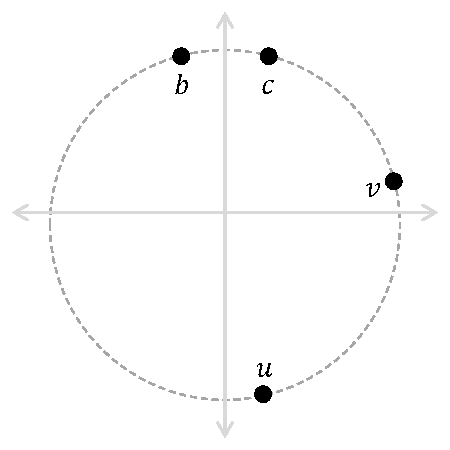
\includegraphics[width=1.5in]{expfig.pdf} \caption{\label{fig:exp} When unsure whether a point is at location $b$ or $c$, the logistic model would strangely prefer comparing it to $u$ and $v$ over $b$ and $c$ themselves.  The exponential model makes this prediction because $(b-c) \cdot (u-v) > (b-c)\cdot (b-c)$.}
\end{SCfigure}

This criterion for evaluating a model, namely the quality of triples it gives rise to, is perhaps an interesting one.

\section{System parameters and quality control}\label{sec:params}
We've described abstractly how our system is implemented.  This
section describes parameters and specifics of our optimization
algorithms and experiments.

Experiments were performed using Amazon's Mechanical Turk web service,
where we defined `Human Intelligence Tasks' to be performed by one or
more users.  Each task consists of 50 comparisons and the interface is
optimized to be performed with 50 mouse clicks (and no scrolling).
The mean completion time was approximately 2 minutes, for which
workers were paid 15 cents (US).  This price was determined based upon
worker feedback.  At 10 cents per task, though workers actively
performed the tasks, some complained about low wages and several
suggested that they be paid 15 cents per task.  At 15 cents per task,
feedback was extremely positive -- the users reported that the tasks
were enjoyable and requested more.  Initial experiments revealed a
high percentage of seemingly random responses, but after closer
inspection the vast majority of these poor results came from a small
number of individuals.  To improve quality control, we imposed a limit
on the maximum number of tasks a single user could perform on any one
day, we selected users who had completed at least 48 tasks with a 95\%
approval rate, and each task included 20\% triples for which there was
tremendous agreement between users.  These ``gold standard'' triples
were also automatically generated and proved to be an effective manner
to recognize and significantly reduce cheating.  The system is
implemented using Python, Matlab, and C, and runs completely
automatically in Windows and Unix.

\subsection{Question phrasing and crowd alignment}
One interesting issue is how to frame similarity questions.  On the
one hand, it seems purest in form to give the users carte blanche and
ask only, ``is $a$ more similar to $b$ than $c$.''  On the other hand,
in feedback users complained about these tasks and often asked what we
meant by similarity.  Moreover, different users will inevitably weigh
different features differently when performing comparisons. 


%For
%example, consider a comparisons of face images, where $a$ is a white
%male, $b$ is a black male, and $c$ is a white female.  Some users will
%consider gender more important in determining skin color, and others
%may feel the opposite is true.  Others may feel that the question is
%impossible to answer.  Consider phrasing the question as follows, ``At
%a {\em distance}, who would you be more likely to mistake for $a$: $b$
%or $c$?''  For any two people, there is presumably some distance at
%which one might be mistaken for the other, so the question may seem
%more possible to answer for some people.  Second, users may more often
%agree that skin color is more important than gender, because both are
%easily identified close up by skin color may be identifiable even at a
%great distance.  While we haven't done experiments to determine the
%importance of question phrasing, anecdotal evidence suggests that
%users enjoy the tasks more when more specific definitions of
%similarity are given.

Two natural goals of question phrasing might be: (1) to align users in
their ranking of the importance of different features and (2) to align
user similarity notions with the goals of the task at hand.  For
example, if the task is to find a certain person, the question,
``which two people are most likely to be (genealogically) related to
one another,'' may be poor because users may overlook features such as
gender and age.  In our experiments on neckties, for example, the task
was titled ``Which ties are most similar?'' and the complete
instructions were:

\begin{quote}
  Someone went shopping at a tie store and wanted to buy the item on
  top, but it was not available. Click on item (a) or (b) below that
  would be the {\bf best substitute}.
\end{quote}




\section{Experiments and Applications}

%4a. floor tiles and/or flags
%first part: learning the human kernel for this
%- example triplets: what mturkers saw, also show how triplets change with adaptivity (vs. random)
%- embedding: projected into 2D (possibly snapped to grid)
%- nearest neighbor examples (when it's done training)
%- attribute discovery: user takes set of embedded "feature vectors," sets up supervised learning problem by labeling subset of training examples that have a %certain attribute (e.g., zig zag pattern), trains SVM to extrapolate to remaining examples; this shows the descriptive power of the embedded representation
%- quantitative plots: triplet preference prediction accuracy vs. time/money invested into crowdsourcing for different adaptive sampling methods and different %fitting methods
%- observed training/run time
%second part: using the human kernel to build a visual search interface
%- describe interactive/sequential search interface with blocks of 9 choices user can click
%- question is: how long/how many clicks does it take to get to desired object
%-- user may expect clustery feel; we need to emphasize that what we're shooting for is smallest number of clicks to get to desired target
%- performance evaluation: number of clicks averaged over many object instances, prediction accuracy for which of the 9 images they click on
%4b-d. more example domains
%- letters a-z?

\begin{figure}
\center{\includegraphics[width=3.2in]{rand_vs_adaptive.pdf}} \caption{\label{fig:YAY} The 20Q plots comparing training based on adaptively selected triples to randomly selected training triples.  The left plot shows the mean predicted log-ranks of randomly chosen objects after 20 randomly chosen questions. The right plot shows the mean predicted log-ranks of randomly chosen objects after 20 adaptive queries.
Plots were generated using the mixed dataset consisting of $n=225$ objects, with 10 initial random triples per object.  In both plots, the performance using $22 = (10 $ random$) + (12$ adaptively chosen$)$ triples was matched using all 35 random triples.  Hence, approximately 60\% more random triples were required to match this particular performance level of the adaptive algorithm.
}
\end{figure}


We experiment on four datasets: (1) twenty-six images of the lowercase roman alphabet (Calibri font) (2) 223 country flag images from flagpedia.net, (3) 433 floor tile images from Amazon.com, and (4)
300 product images from an online tie store also hosted at Amazon.com. We also consider a hand-selected ``mixed'' dataset consisting of 225 images: 75 ties, 75 tiles, and 75 flags.  Surprisingly, it seems
that for these datasets about 30-40 triples per object suffice to
learn the Crowd Kernel well. Figure \ref{fig:YAY} shows the results on the mixed dataset, comparing the 20Q metric (described below) trained on random vs.~adaptive triples.  For both adaptive and random questions, for certain performance levels, one requires about 60\% more random queries than adaptive queries.  Given very little data or a lot of data, one does not expect the adaptive algorithm to perform significantly better.

Figure \ref{fig:adaptive-trips} shows the adaptive triples selected on
an illustrative dataset composed of a mixture of flags, ties and
tiles.

For ease of implementation, we assume all users are identical.  This
is a natural starting point, especially given that our main focus is
on active learning.


\begin{figure}
\center{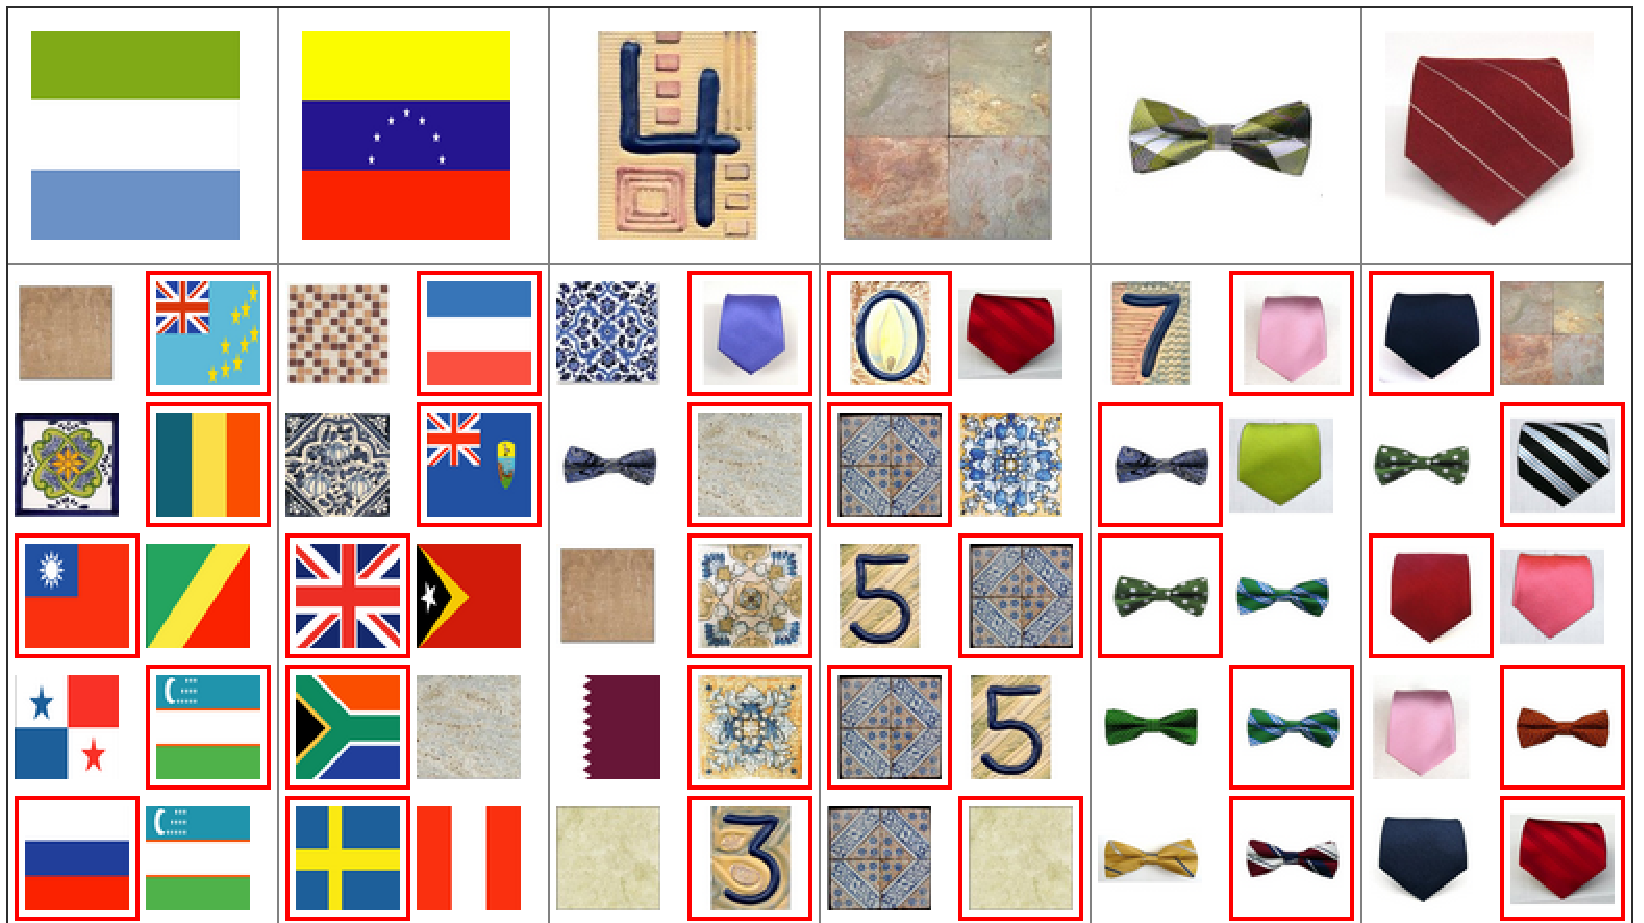
\includegraphics[width=3.4in]{adaptive_combo.pdf}} \caption{\label{fig:adaptive-trips} Six objects in the mixed dataset along with the adaptive pairs to which that object was compared, below, and user selections in red.  The first pair below each large object was chosen adaptively based upon the results of ten random comparisons.  Then, proceeding down, the pairs were chosen using the ten random comparisons plus the results of the earlier comparisons above.}
\end{figure}
\begin{figure}
{\center 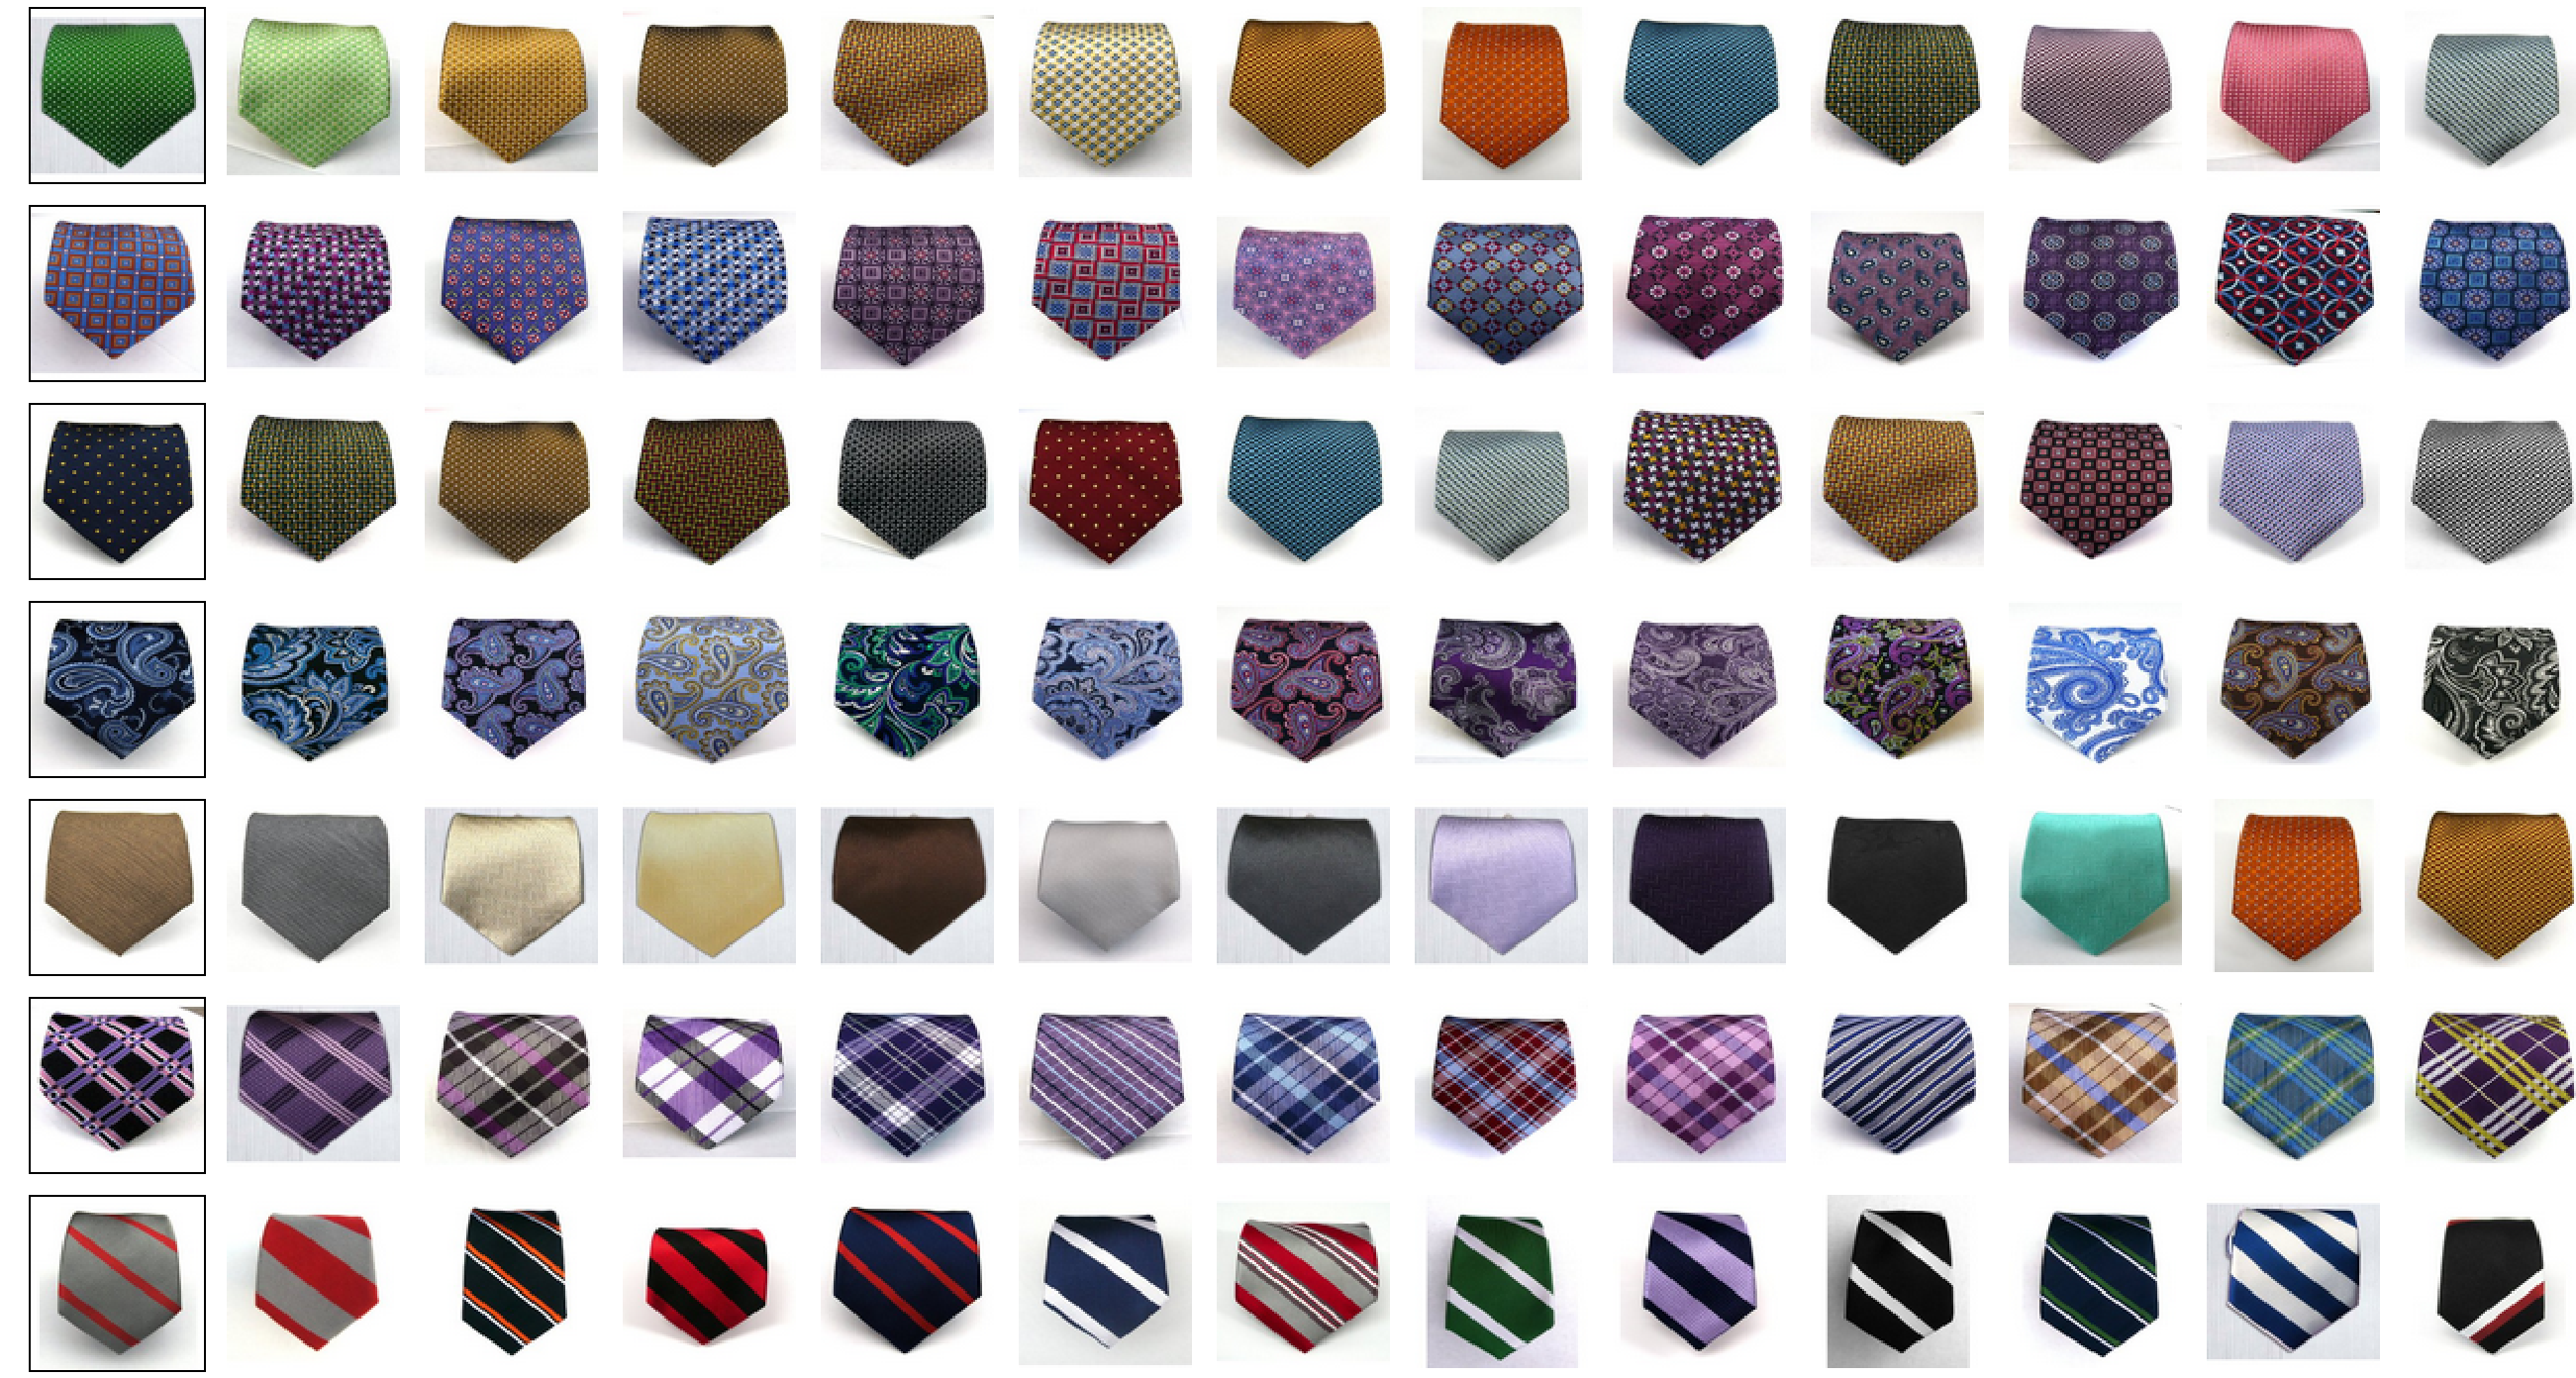
\includegraphics[width=3.4in]{neckties_neighs.pdf}} 
\caption{\label{fig:nn} Nearest-neighbors for some neckties from the tie-store dataset.  Nearest neighbors are displayed from left to right.  Note that neck ties were never confused for bow ties, tie clips or scarves.
}
\end{figure}
\begin{figure}
{\center 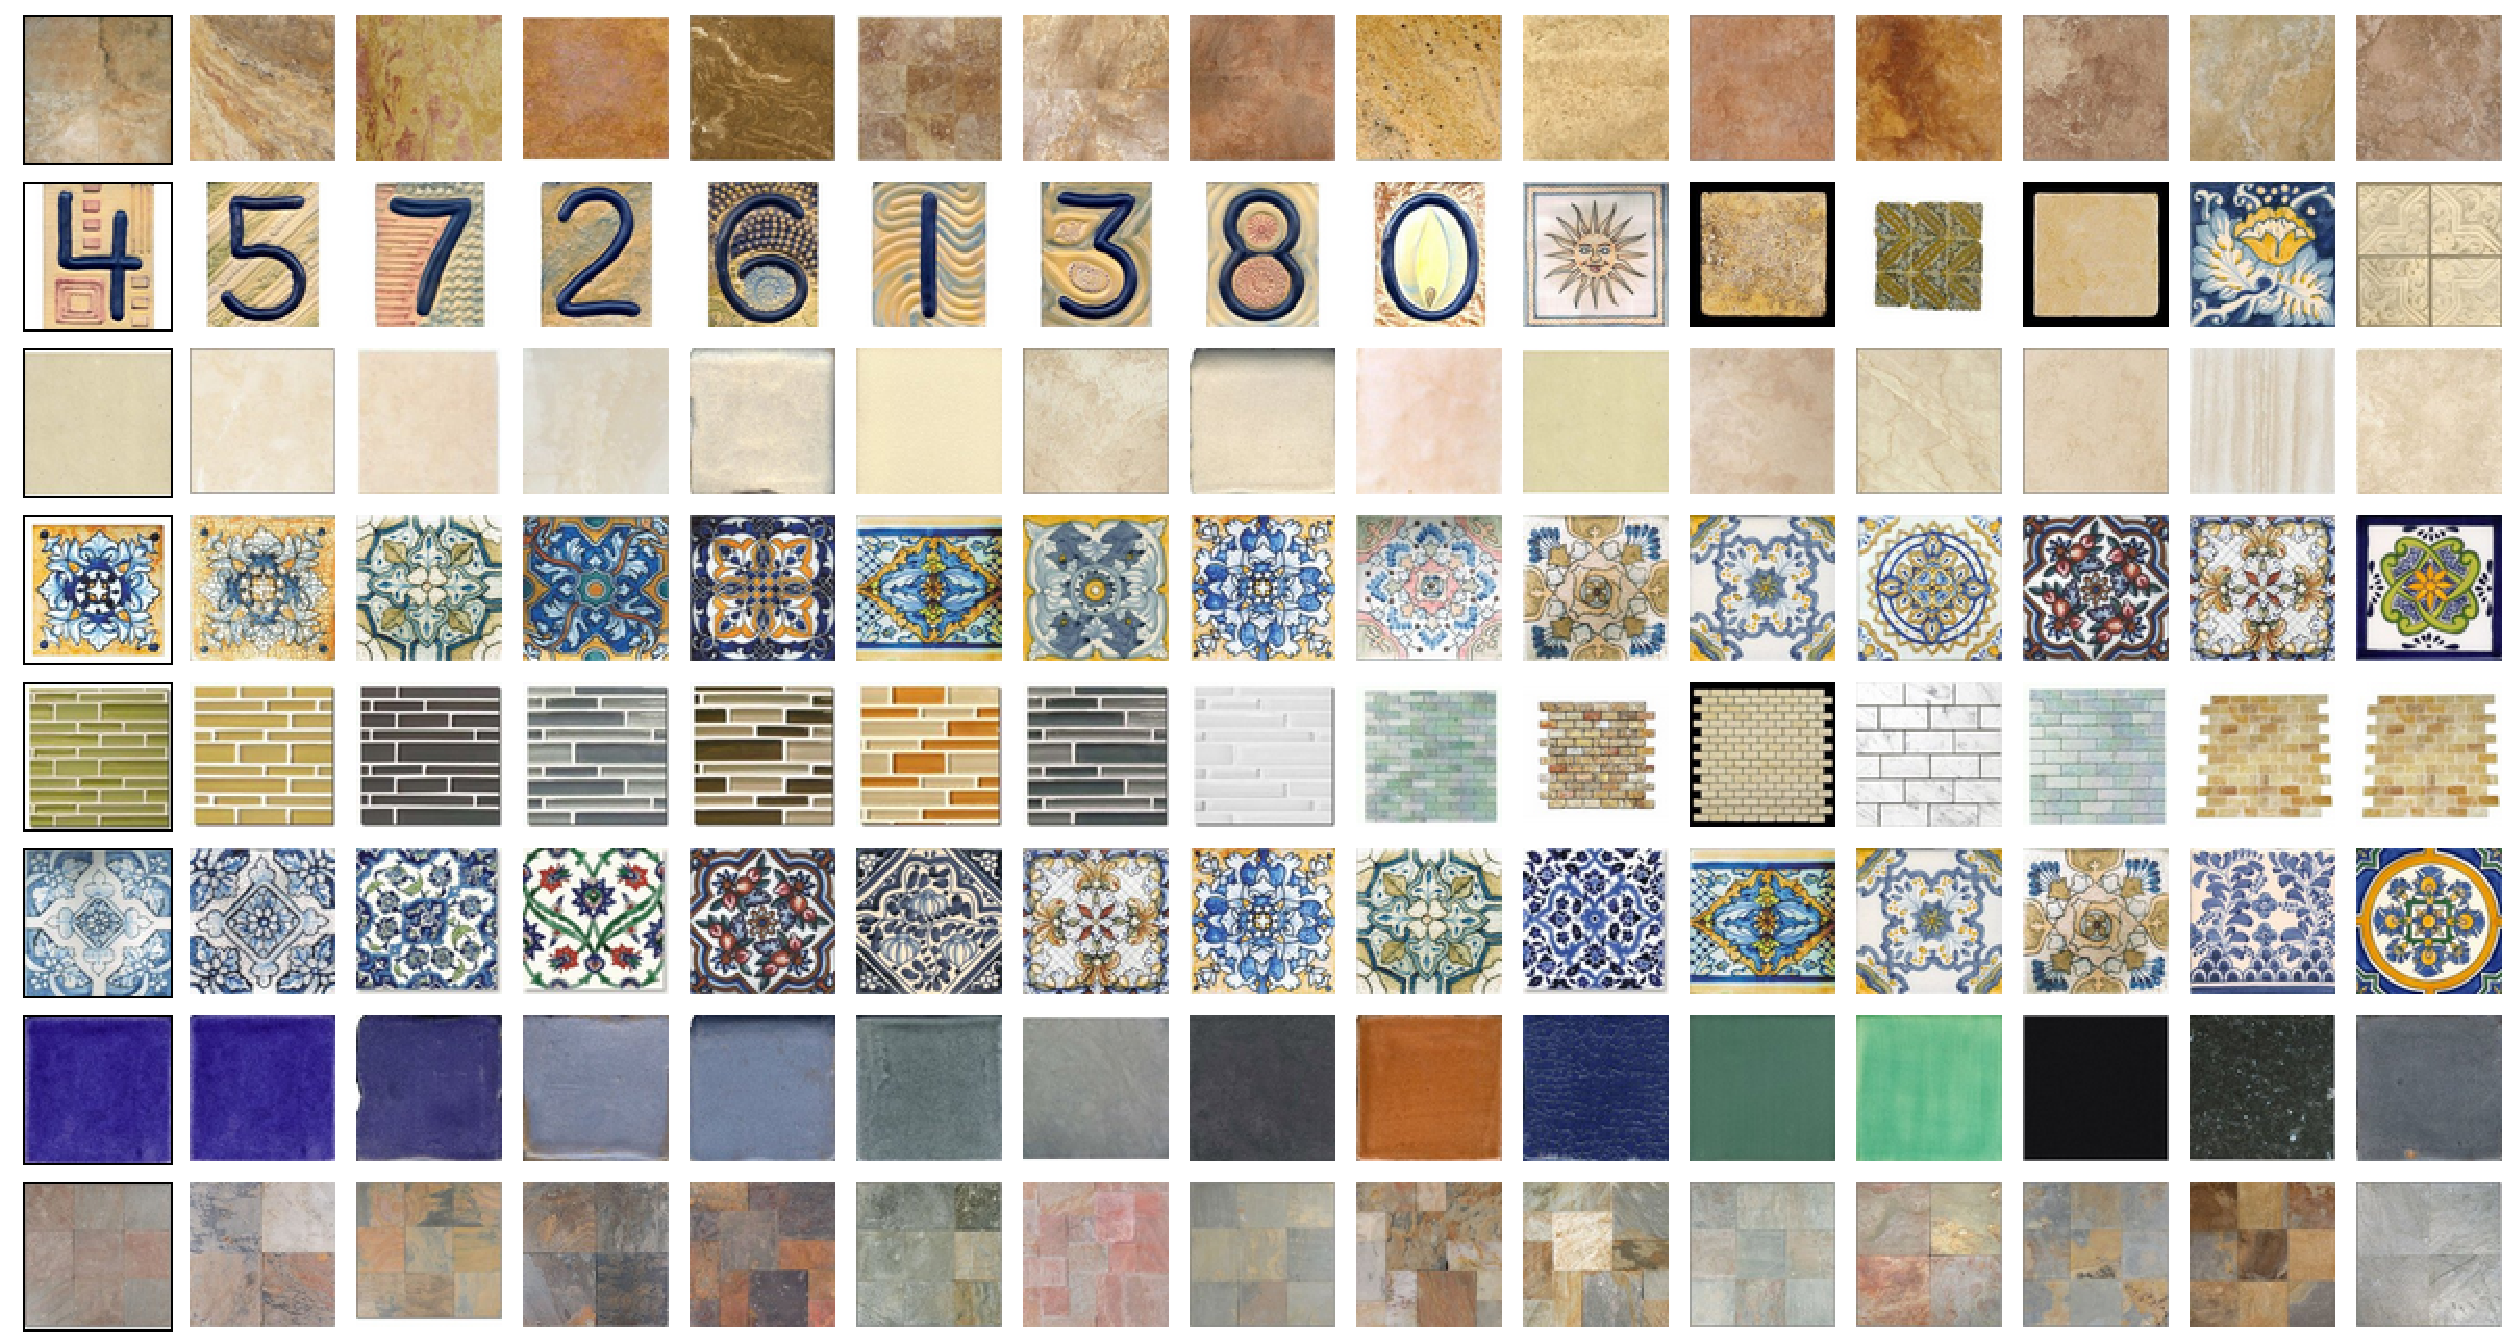
\includegraphics[width=3.4in]{tiles_neighs.pdf}} \caption{\label{fig:nn-tiles} Examples of nearest neighbors for floor tiles.}
\end{figure}
\begin{figure}
{\center 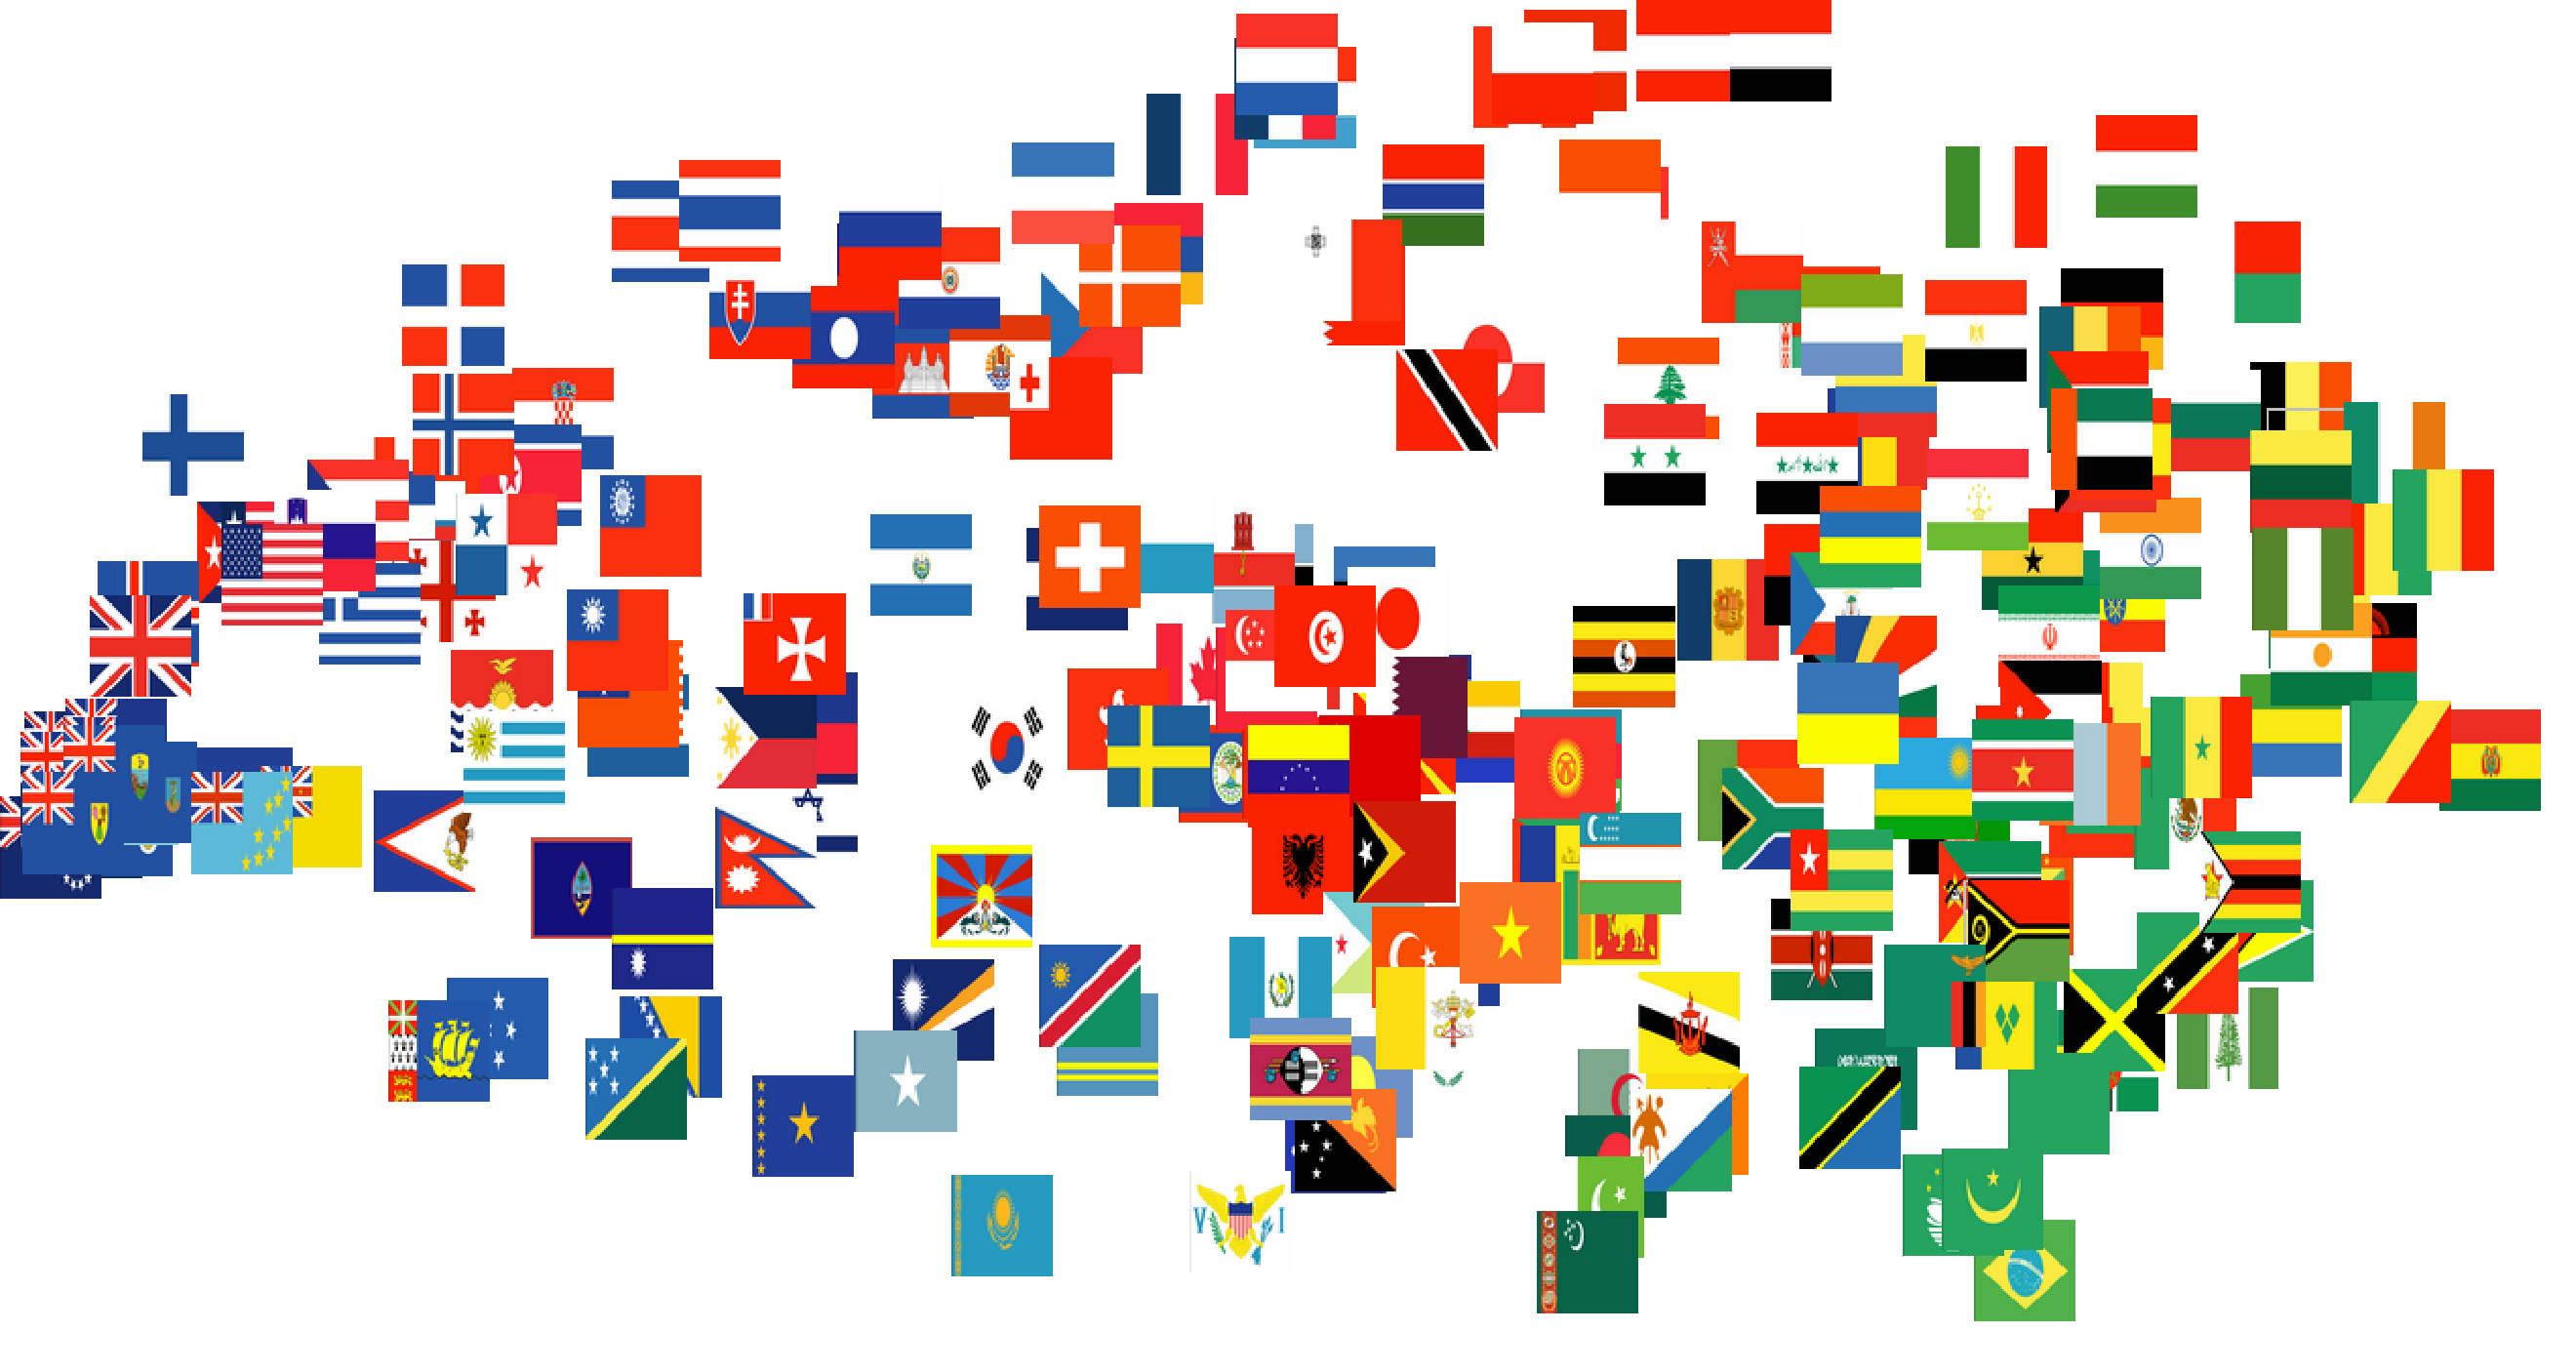
\includegraphics[width=3.5in]{flags_pca.pdf}} \caption{\label{fig:flagspca} The flag images displayed according to their projection on the top two principal components of a PCA.  (The principal component
is the horizontal axis.)}
\end{figure}

\subsection{20 Questions Metric}
Since one application of such systems is search, i.e., searching for an item that a user knows what it looks like (we assume that the user can answer queries as if she even knows what the store image looks like), it is natural to ask how well we have ``honed in'' on the desired object after a certain number of questions.  For the 20 Questions (20Q) metric, imagine that the user has selected a secret object in the database, uniformly at random, and the system is allowed to query 20 triples (as in the game ``20 Questions''), after which it produces a ranking of items in the database, from most to least likely.  The metric is the average $\log$ of the position of the random target item in this list.  The $\log$, common in ranking, reflects the idea that the position of lower-ranked objects is less import -- it weights moving an object from position 2 to 4 as important as moving an object from position 20 to 40.  (We note that we observed similar behavior for the expected position metric.)  This metric is meant to roughly capture performance, but of course in a real system users may not have the patience to click on twenty pairs of images and may prefer to choose from larger sets. (Our GUI has the user select one of 8 or 9 images, which could potentially convey the same information as 3 binary choices.)  Now, the questions that the system asks could be random questions, which we refer to as the 20 Random Questions metric, or adaptively chosen, for the 20 Adaptive Questions metric.  In the later case, the same maximum information-gain criterion is used here as in the adaptive triple generation algorithm, relative to whichever model was learned (based on random or adaptively selected training triples).


\subsection{Using the Kernel for Classification}

The learned Kernels may be used in a linear classifier such as a
support vector machine.  This helps elucidate which features have been used
by humans in labeling the data.  In the experiments below, an unambiguous subset of the images were
labeled with binary $\pm$ classes. For example, we omitted the letter {\em y} in labeling vowels and consonants ({\em y} was in fact classified as a consonant, and {\em c} was misclassified as a vowel), and we selected only completely striped or unstriped flags for flag stripe classification.  The SVM-Light \cite{Joachims98} package was used with default
parameters and its leave-one-out (LOO) classification results are reported.


Note that the low error rates are heavily influenced by the fact that we hand-selected ``easy'' subsets of objects to label.  The selection was based on how unambiguous the objects were, with respect to the desired label, and not related to the target kernel.

\begin{tabular}{|l|l|l|}
 \hline
 Dataset & Feature & LOO error rate \\
 \hline
 \hline
Tiles & Ornate & 4.1\% \\
Ties & Bow tie vs.~neck tie & 0.0\%\\
Ties & Multicolor vs. plain & 0.5\%\\
Flags & Striped & 0.0\%\\
Letters & Vowel & 4.0\%\\
Letters & Short/tall & 5.3\%\\
\hline
\end{tabular}


\subsection{Visual Search}
We provide a GUI visual search tool, exemplified in Figure
\ref{fig:tilestree}. Given $n$ images, their embedding into $\reals^d$
and the related probabilistic model for triples, we would like to help
a user find either a particular object she has in mind, or a similar
one. We do this by playing ``20 Questions'' with 8 or 9-tuple queries, generated by an information-gain 
adaptive selection algorithm very similar to the one described in Section \ref{sec:ada}.

\section{Conclusions}
In this work, we provide an algorithm and an end-to-end system for constructing an embedding of
objects in to Euclidean space (and hence also an $n \times n$ similarity matrix) from {\em adaptively chosen} crowdsourced
similarity comparisons alone.  Our algorithm requires no image features to be extracted and hence can be used across a number of domains.
The learned kernel can be used in a kernel-based learning algorithm, such as SVM, to demonstrate that the kernel has indeed captured features of interest to people.  An application is given for similarity-based search.  

\bibliography{sim}
\bibliographystyle{icml2011}

\end{document}


% This document was modified from the file originally made available by
% Pat Langley and Andrea Danyluk for ICML-2K. This version was
% created by Lise Getoor and Tobias Scheffer, it was slightly modified
% from the 2010 version by Thorsten Joachims & Johannes Fuernkranz,
% slightly modified from the 2009 version by Kiri Wagstaff and
% Sam Roweis's 2008 version, which is slightly modified from
% Prasad Tadepalli's 2007 version which is a lightly
% changed version of the previous year's version by Andrew Moore,
% which was in turn edited from those of Kristian Kersting and
% Codrina Lauth. Alex Smola contributed to the algorithmic style files.


